\chapter{The Workhorses of Electronic Structure Theory}
\label{chap:gw}
\noindent
\section{Introduction}
In this chapter we discuss the principles underlying Density Functional
Theory (DFT) within the local density approximation (LDA).
We also discuss the GW\footnote{Initialism to be explained in subsequent sections.} method
which provides us with a systematic way of improving on the local density approximation.
These tools have been called the `workhorses' of theoretical materials science\cite{sohrab17}.
They are workhorses because they shoulder much of the computational heavy lifting that needs
to be done to obtain an accurate picture of how electrons arrange themselves in materials.
They also provide the means for calculating the diverse range of material properties 
that arise from these arrangements.

The guiding principle of this chapter is we wish to start 
from the `best possible' ground-state description.
That is a ground-state that can be calculated precisely according to a 
well defined variational principle. 
This ground-state may come from a Hartree-Fock ground-state, or a simple
DFT+LDA ground-state, we may even choose our
ground-state to be a superposition of atomic orbitals. The only further requirement
we impose is that whichever ground-state we choose, barring singular cases,
we should be able to define an iterative scheme that improves the correspondence
between the model and the physical data. We will use the GW approximation to accomplish this.

The approach to the GW scheme taken here is that it is essentially a perturbation scheme.
Given an arrangement of electrons we are interested in how their motion is correlated.
That is if we alter the electronic density around one atom can we calculate the changes induced in 
the electronic density localized around another atom in the system?
If we are smart about what center (ground-state) we choose to expand around we may
expect more or less rapid convergence to a stable solution of this problem. We may also eliminate
the ambiguity in our calculations that arises from our choice of ground-state.

Having considered the different ways of obtaining an initial description of our
electronic system and the iterative approach for improving that description we need
to make the connection with the tight-binding recursion method introduced in the previous chapter. 
We need to transform the ground-state properties we can compute ab initio, 
into a framework capable of being written purely in terms of local interactions.
The Harris-Foulkes functional provides us with the means to accomplish this. 

In the next chapter we will use the theory developed here
to build local electronic models for some interesting 
physical systems.

\section{Density Functional Theory}
\subsection{Hohenberg-Kohn theorem}
\label{sec:hohnkohn}
Modern Density Functional Theory (DFT) has its foundations in the 
papers of Hohenberg and Kohn~\cite{hohenbergkohn64}, and Kohn and Sham~\cite{kohnsham65}.
People like DFT because it provides a means for obtaining the ground-state energy of an
interacting system of electrons without having to work directly with a high dimensional
wave function.

In 1964 Hohenberg and Kohn~\cite{hohenbergkohn64} presented a proof 
that the ground-state energy of a system of interacting electrons
in a fixed external potential is a unique functional of the 
electronic density $n(\r)$. This is a theorem which, over time,
has launched a thousand (millions) of ships (calculations).

According to Hohenberg and Kohn the ground-state energy, as a 
functional of the density, can be written:
%
\begin{equation}
\label{eq:hkenergy}
E[n] = \int v(\r) n(\r)d\r + F[n].
\end{equation}
%
Eq.~\ref{eq:hkenergy} divides the total energy functional $E[n]$ into different contributions.
$\int v(\r)n(\r)d\r$ is the energy contribution from the external potential $v(\r)$. $F[n]$ 
is a functional containing the Hartree energy along with all
the remaining electron-electron interaction effects.
%
If an explicit expression for $F[n]$ is provided, then 
Eq.~\ref{eq:hkenergy} can be minimized with respect 
to variations of the density $\delta n$.

To prove this theorem Hohenberg and Kohn began 
from a Hamiltonian for the interacting electronic system of the form:
%
\begin{equation}
\hat{H} = \hat{H}_{0} + \hat{H}_{\rm{int}} + v(\r),
\end{equation}
%
where $\hat{H}_{0}$ is the kinetic energy, $\H_{\rm{int}}$ is the electron-electron Coulomb repulsion
and $v(\r)$ is the local external potential. Given the particular Hamiltonian $\H$, and its associated
ground-state electronic wave function $\Psi$, the ground-state energy of the system is: 
%
\begin{equation}
E = \bra \Psi | \H | \Psi \ket.
\end{equation}
%
The proof of the Hohenberg-Kohn Theorem is carried out using a \textit{reductio ad absurdum} 
argument. Initially it is assumed that two external potentials, which differ by no more than
a constant, can give rise to the same ground-state electron densities. The two potentials
give rise to two different Hamiltonians, with different ground-state wave functions. It
can then be demonstrated that this gives rise to a contradiction in the ground-state
energies for the two different external potentials. The only way to resolve the contradiction
is to accept that the external potential is uniquely determined by the ground-state density to 
within a constant. The corollary of this is also true and the Hamiltonian is uniquely determined
as a functional of the ground-state density~\cite{martin}. 
The original proof is valid for non-degenerate grounds states, 
and the use of constrained searches generalized the proof
to arbitrary ground-states~\cite{levy79, levy82, lieb83}.

The Hohenberg-Kohn theorem gives us an existence proof:
there is a universal functional of the electronic density
from which we can obtain information about the ground-state properties
of a system given an external potential.
We are also in possession of another constraint: the conservation of charge.
We may combine the total energy functional with 
the charge density constraint using a Lagrange multiplier:
%
\begin{equation}
\frac{\delta}{\delta n(\r)} \left[E[n(\r)] - \lambda(\int n(\r)d\r - N)\right] = 0,
\end{equation}
%
which leads to:
%
\begin{equation}
\frac{\delta E[n(\r)]}{\delta n(\r)}= \lambda.
\end{equation}

Once armed with some approximation to the exchange-correlation functional, a computer, 
and the comforts of a well defined variational principle and conservation law,
the materials scientist is in a position to go out and do a significant amount of damage. 

\subsection{Kohn-Sham Theory: Partially Restoring the Orbitals}
\noindent
To proceed from Hohenberg-Kohn we need a practical way of performing calculations.
We need to choose some initial charge density and we need to approximate the 
exchange-correlation contribution to the total energy.
Kohn and Sham provided a reformulation of the problem which enables us to 
do both these things. They began by considering an auxiliary set of 
non-interacting electrons\cite{kohnsham65}, $\psi_{i}(\r)$, 
which have the same charge density as the true interacting system:
%
\begin{equation}
\label{eq:density}
n(\r) = 2\sum^{\rm{n_{occ}}}_{i=1} \psi_{i}^{*}(\r)\psi_{i}(\r).
\end{equation}
%
Where $\rm{n_{occ}}$ is the number of occupied electronic states in the system and the
factor of two accounts for spin degeneracy. Eq.~\ref{eq:density} implies that the many-electron
wave function is a single Slater determinant. 

The Hamiltonian for the non-interacting electronic
states is chosen such that it is composed of the kinetic energy operator for 
the non-interacting electrons (which is important as we shall see), 
and a potential that is purely local:
%
\begin{equation}
\label{eq:lda}
\H^{\rm{KS}} = -\frac{1}{2}\nabla^{2} + \sum_{j}V_{\rm ion}(\r-\mathbf{R}_{j}) + V_{\rm H}(\r) + V_{\rm xc}(\r).
\end{equation}
%
Here $V_{\rm ion}(\r-\mathbf{R}_{j})$ is the Coulomb potential felt by an
electron at point $\r$ from a nucleus at point $\mathbf{R}_{j}$.
The term $V_{\rm{H}}(\r)$ is the Hartree potential:
%
\begin{equation}
V_{\rm{H}}(\r) = \int \frac{n(\r')}{|\r-\r'|}d\r',
\end{equation}
%
and the remaining term is the exchange and correlation potential $V_{\rm{xc}}$. 

We can solve a set of eigenvalue equaionts:
%
\begin{equation}
H^{\rm KS} \psi_{i} = \epsilon_{i}
\end{equation}

The thinking is that we may now write out total energy as:
%
\begin{equation}
E[n] = \int v(\r)n(\r)d\r + T[n] + E_{\rm H}[n] + E_{\rm xc}[n]
\end{equation}

Where we can compute $T[n]$ directly: 
%
\begin{equation}
T[n] = \sum_{i} \epsilon_{i} - \int d\r n(\r) \left[ v(\r)  + V_{\rm H}[n] + \frac{\delta E_{\rm xc}[n]}{\delta n} \right]
\end{equation}

If an explicit functional dependence on $n(\r)$ for $E_{\rm{xc}}$ is provided 
we can then seek an energy minimum for the non-interacting electronic system 
by minimizing the variation in the total energy with respect to the density:
%
\begin{equation}
\frac{\delta E^{\rm{KS}}[n]}{\delta \psi^{*}_{i}} = 0,
\end{equation}
%
and ensuring that the orthogonality constraints between the wavefunctions:
%
\begin{equation}
\bra \psi_{i} |\psi_{j}\ket = \delta_{i,j},
\end{equation}
%
are satisfied.
 
The Kohn-Sham Hamiltonian is determined by the electronic density $n(\r)$; the electronic density is 
defined by the single-particle wavefunctions, $\psi_{n}(\r)$ in Eq.~\ref{eq:density}; and, 
finally, the single particle wavefunction are defined by the solutions of the equation:
%
\begin{equation}
\label{eq:kseq}
\H^{\rm{KS}}\psi_{n}(\r) = \epsilon_{n}\psi_{n}(\r).
\end{equation}
%

The dependency of the Hamiltonian on the density means obtaining the Kohn-Sham 
wavefunctions and eigenvalues requires a self-consistent
procedure. 

The Kohn-Sham formulation is in the spirit of the time honoured 
trick of regrouping terms over and over again to try and squeeze our 
ignorance into a smaller space. 

In this case the by solving the eigenvalue problem for the non-interacting
electronic system we
re-introduces the explicit inclusion of an orbital angular momentum 
character, s,p,d etc., to the kinetic
energy term (which we mentioned was important a little earlier). 
It is this kinetic energy term which prevents the electrons from piling into 
narrow regions of space and encourages the electrons to diffuse throughout the system.

We maintain explicit representations of the Hartree and the electron-ion contributions 
that can be computed directly. If our non-interacting system kinetic energy
is a fair guess at that of the the true interacting electronic system this means most of 
our remaining ignorance has been pushed into $E_{xc}[n]$. We will
approximate this term with the local density approximation. 
 
\subsection{The Local Density Approximation}
\noindent
\label{sec:thelda}
The practical success of DFT is largely determined by our ability to
find an adequate approximation to the exchange and correlation functional.
For many ground-state properties the Local Density Approximation (LDA) 
has proven to be good enough. In this scheme the exchange and correlation energy
is written:
%
\begin{equation}
E_{\rm{xc}}[n(\r)] = \int \epsilon_{\rm{xc}}(n(\r))n(\r)d\r,
\end{equation}
%
where $\epsilon_{\rm{xc}}(n(\r))$ is the energy per electron at a point $\r$,
which depends only upon the density $n(\r)$ \textit{as calculated for an homogeneous electron 
gas}. The exchange and correlation potential 
can be obtained from the exchange correlation energy via:
%
\begin{equation}
\label{eq:kohnshampot}
V_{\rm{xc}}(\r) = \frac{\delta E_{\rm{xc}}[n(\r)]}{\delta n(\r)}.
\end{equation}
%

Intuitively the rule is the following: where a little charge has accumulated
the LDA contribution of this charge will lower the total energy. In the self-consistent
scheme this means at the next iteration it may well be favourable to add a little more
charge to that region, and in this way, the LDA encourages the pile up of electronic charge
in bonds. It is sometimes said that the LDA tends to overbind systems.

A number of parametrizations for the function $\epsilon_{xc}(n(\r))$ exist.
The earliest was given by Wigner\cite{wigner34a} who provided an interpolation formula
between the exchange-correlation functional for the high and low density electron gas.
The first numerical parameterizations of the correlation energy were based
on fitting a curve to Monte Carlo calculations of the correlation energy
of the homogeneous electron gas\cite{ceperly80, vosko80, 
perdew81, perdewwang92}. There are additional approximations to the exchange 
correlation function which incorporate information about the gradient of the
electronic density or elements of exact exchange\cite{becke88, perdew96, becke93, becke93b}
some of which improve upon the aforementioned overbinding tendency at the expense of
increased meddling.

\subsection{Anticipating $GW$}
\cite{kohnshamII}
The generalization of the exchange and correlation operator beyond the LDA 
in order to allow for non-locality and the energy dependence of the exchange and
correlation potential is also discussed in, the relatively overlooked, Ref.~\cite{shamkohn66}. 
In this work Kohn and Sham rewrite Eq.~\ref{eq:kseq} following Refs.~\cite{schwinger51, hedin65}:
%
\begin{equation}
\label{eq:qpeq}
\left[-\frac{1}{2}\nabla^{2} + V_{\rm{ion}}(\r) + V_{\rm{H}}(\r)\right]\psi_{n}(\r) + \int \Sigma(\r,\r';E_{n})\psi_{n}(\r') d\r' = E_{n}\psi_{n}(\r).
\end{equation}
%
Here the quantity $\Sigma(\r,\r';\omega)$ is a non-local and energy dependent
operator which encodes all the electronic correlations present in the system. 

In terms of total energy of the system we can write:
%
\begin{equation}
\label{eq:shamschlut}
E = E_{NN} + \sum_{n} E_{n} - \frac{1}{2}\int V_{N}(\r)\rho(\r)d^{3}\r
-\frac{1}{2}\int\int\sum_{n} \psi_{n}^{*}(r)V_{xc}(\r,\r';E_{n})\psi_{n}(\r')d^{3}\r d^{3}\r',
\end{equation}
%
which provides a natural link in our discussion of DFT to methods
based on many body perturbation theory \cite{shamschlut83} and the $GW$
approximation.

%Although adequate for describing structural properties the 
%LDA has difficulty describing the electronic excitations 
%of a many electron system.
%This is partly due to deficiencies inherent in the approximations
%to the exchange correlation potential, and to the
%inherent discontinuity upon the addition or
%removal of an electron present in the
%exact functional \cite{perdew83, sham83, godby86}. There
%are a number of possible approaches for extending the DFT
%formalism to access excited state properties. Hybrid functionals
%~\cite{rinke05, friedrich12} and $\Delta$SCF methods~\cite{gunnarsson76, jones89}
%go someway towards providing a formalism for accurately calculating
%excitation energies. 

\section{$GW$}
The $GW$ formalism takes its name from the the Green's function, denoted~$G$, and the 
screened Coulomb interaction,~$W$\cite{hedin65}. The $GW$ formulation is due
to Lars Hedin with the presidential address coming in:
``New Method for Calculating the One-Particle Green's Function
with Application to the Electron-Gas Problem.''~\cite{hedin65}. 

In this work Hedin developed a
self-consistent system of equations for including all the interaction effects
in a many electron system. Hedin describes the
connection between his work and the development of Green's
functions methods in the field of quantum electrodynamics by Schwinger in Ref.~\cite{schwinger51}.
An early review of the applications of Green's function methods and
Feynman diagrams to the many electron problem was given in Ref.~\cite{pratt63}. 
The procedure has been extensively studied in the 
intervening thirty years and Refs.~\cite{aulbur00, aryasetgunnarsson98, onida02}
provide a review of the contemporary state of the field.

We begin by discussing the analytic properties of the interacting and
non-interacting Green's function and how the Green's function encodes information about
the many-body excited electronic states. To derive Hedin's equations, from which
the $GW$ approximation follows, we examine the equation of motion for the Green's function and
construct a closed loop of equations which contain all the effects of the
electron-electron interaction. 

DFT lets us pass from the many-body wave function, which is too difficult to work with,
to the electronic density which is more convenient but slightly too simple. The Green's
function is the Goldilocks representation containing more information than the density,
less than the total wavefunction, and is just about manageable to work with.

\subsection{Definition of the Green's function}
\label{subsec:defgreenfun}
To begin the discussion of the $GW$ approximation we introduce the Green's function. 
The Green's function is defined as:
%
\begin{equation}
\label{eq:green0}
G(\r,t,\rp,t') = \bra N|\hat{T}\left[\field(\r,t)\cfield(\rp,t')\right]|N \ket,
\end{equation}
%
$\hat{T}$ is the time ordering operator ensuring events at time $t$ occur
after event $t'$. $\cfield$ and $\field$ are the fermion 
creation and annihilation field operators:
%
\begin{equation}
\field(\r,t) = \sum_{n} \phi_{n}(\r) c_{n}(t),
\end{equation}
%
and 
%
\begin{equation}
\cfield(\r,t) = \sum_{n} \phi^{\star}_{n}(\r) c^{\dagger}_{n}(t),
\end{equation}
%
where $c^{\dagger}_{n}(t)$ and $c_{n}(t)$ are creation 
and annihilation operators, and $\phi_{n}(\r)$ are 
the single particle wave functions, these could be Kohn-Sham wavefunctions. 
The ground-state wave functions can be obtained from a DFT calculation. 
Note the time dependence is included in the creation and 
annihilation operator rather than the wave function. $|N\ket$ represents 
the electronic ground-state wave function for a system of $N$ electrons.

The time ordering operator can be expanded for
the single particle Green's function to provide:
%
\begin{eqnarray}
\label{eq:green}
G(\r,t,\rp,t') & = & -i\Theta(t-t') \bra N|\field(\r,t)\cfield(\rp,t') |N \ket \nonumber \\
	  	 	   &   & +i\Theta(t'-t) \bra N|\cfield(\rp,t')\field(\r,t) |N \ket. 
\end{eqnarray}
%
In Eq.~\ref{eq:green} $\Theta$ is the Heaviside step function. This ensures the causality 
of the Green's function. Physically we can interpret the role of the Heaviside step function
as differentiating between two scenarios. When  $(t-t')>0$ the situation 
corresponds to the matrix element with the many-body wavefunction 
of an electron added to the system at the time $t'$ in position $\r'$, and subsequently removed
from the system at $\r,t$. For the case $(t'-t)>0$ the Green's function describes the propagation
of a hole.

%
Let us dwell a little bit longer on what Eq.~\ref{eq:green} represents. 
Consider the following expression:
\begin{equation}
P(\r,t,\rp,t') = |\bra N|\cfield(\r',t')\field(\r,t)|N\ket|^{2} \qquad t'>t,
\end{equation}
%
which is to be interpreted as denoting the probability that if we remove an electron from the 
position eigenstate $\r$ at time $t$, then, the remaining hole in the electron liquid, 
which plays a similar role to a bubble in a liquid, will propagate to the space-time point $\r',t'$. 
Reversing the time arguments and field operators would correspond to the 
addition of an electron at point $\r',t'$ and removing it at point $\r,t$.
 
There is another useful limit to consider.
Let $\r' \rightarrow \r$ and $t' \rightarrow t^{+}$ 
in Eq.~\ref{eq:green}; in this case the Green's function reduces to the 
charge density of the system.\footnote{$t^{+} = t + \delta$, the 
current time plus an infinitesimal; this is to avoid confusion 
with the definition of, $\Theta$, the Heaviside step function.}

In the case of a non-interacting single-particle Hamiltonian 
the time-dependence of the field operators can be expressed in terms of the 
single-particle eigenvalues, $\epsilon_{n}$, as:
%
\begin{equation}
\label{eq:spoper}
\cfield(\r,t) = \sum_{n} \phi^{*}_{n}(\r)e^{-i\epsilon_{n}t} c^{\dagger}_{n}.
\end{equation}
%
By replacing Eq.~\ref{eq:spoper} inside Eq.~\ref{eq:green} we find:
%
\begin{align}
\label{eq:nonintergr}
G(\r,t,\rp, t') = -i\Theta(t-t')\sum_{\epsilon_n>\epsilon_{f}}\phi_{n}(\r)\phi^{*}_{n}(\rp)e^{-i\epsilon_{n}(t-t')} \nonumber \\
	        			  +i\Theta(t'-t)\sum_{\epsilon_n<\epsilon_{f}}\phi_{n}(\r)\phi^{*}_{n}(\rp)e^{-i\epsilon_{n}(t-t')}.
\end{align}
%
Therefore in this case the Green's function separates naturally into 
two contributions, the first term in Eq.~\ref{eq:nonintergr} coming
from the non-interacting unoccupied electronic states of the system, the second term 
coming from the non-interacting occupied electronic states of the 
system ($\epsilon_{f}$ denotes the energy of the highest occupied state). 

A Fourier transform of Eq.~\ref{eq:nonintergr} then yields the pole structure in 
Fig.~\ref{fig:greenpoles}. In an extended system the set of poles will merge into
branch cuts similarly positioned in the complex plane.
This will be discussed further in the next section
in the context of the interacting Green's function.

\subsection{Analytic structure of the Green's function}
\noindent
The Green's function has two particularly useful properties. 
The first is it effectively encodes all the response properties of the 
system to an external perturbation. The second is that the 
poles of the Green's function in the frequency domain, are
equal to the energies required to excite the $N$ electron system to
a particular state of the $N+1$ or $N-1$ electron system.
%
\begin{figure}[tb]
\begin{center}
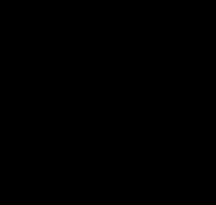
\includegraphics[scale=1.0]{./gw/greenpoles.pdf}
\end{center}
\caption{\small \label{fig:greenpoles} Pole structure 
of the Green's function. The occupied electronic states are
slightly above the real frequency axis and below the chemical 
potential $\mu$, the unoccupied states are located above the Fermi
level and slightly below the real axis. The poles of the Green's 
function correspond to the addition/removal energies 
in the system. This example is for a system with a discrete series of 
excitations and an energy gap between occupied and unoccupied states
of $E_{g}$.}
\end{figure}
%
To demonstrate this it is necessary to Fourier transform the Green's function
from the time domain to the frequency domain. This can be accomplished by 
rewriting the field operators in the Heisenberg representation:
%
\begin{equation}
\label{eq:heisenop}
\cfield(\r,t) = e^{i\hat{H}t}\cfield(\r) e^{-i\hat{H}t}.
\end{equation}
%
We then introduce a complete set of states which describe all the possible 
intermediate excitations of the system to $N'$ particles 
and their $s$ excited states,~$|N',s\ket$:
%
\begin{equation}
\label{eq:compstates}
\sum_{s}|N', s\ket \bra N',s| = \I,
\end{equation}
%
where $\I$ is the identity matrix.
We also note that:
%
\begin{equation}
H|N,s\ket = E^{s}_{N}|N,s\ket.
\end{equation}
%
%
If one inserts Eqs. \ref{eq:heisenop} and \ref{eq:compstates} into Eq.~\ref{eq:green} it is possible 
to write the Green's function in the time domain as:
%
\begin{align}
\label{eq:grtimedom}
G(\r,t,\rp,t') & = & \sum_{s} -i\Theta(t-t') e^{i(E^{0}_{N} - E_{N'}^{s})(t-t')}\bra N|\field(\r)|N',s\ket\bra N',s|\cfield(\r')|N\ket \nonumber \\
	  &+ & \sum_{s} i\Theta(t'-t) e^{-i(E_{N}^{0} - E^{s}_{N'})(t-t')}\bra N|\cfield(\r') |N',s\ket \bra N',s|\field(\r)| N \ket.
\end{align}
%
Now Eq.~\ref{eq:grtimedom} gives the Green's function in the time domain and the arguments depend 
only on differences in time $t-t'$. By introducing the time variable $\tau = t-t'$ it is 
straightforward to define a Fourier transform:
%
\begin{equation}
G(\r,\r';\omega) = \frac{1}{2\pi} \int_{-\infty}^{\infty} G(\r,\r,\tau) e^{i\omega\tau} d\tau,
\end{equation}
%
and represent the Green's function in the frequency domain:
%
\begin{eqnarray}
\label{eq:greenfreq}
G(\r,\rp;\omega) & = &\sum_{s} \frac{\bra N|\field(\r) |N',s\ket \bra N',s|\cfield(\r')| N \ket}{\omega - (E^{s}_{N'} - E^{0}_{N}) + i\delta} \nonumber \\
	  		     & - & \sum_{s}\frac{\bra N|\cfield(\r') |N',s\ket \bra N',s|\field(\r)| N \ket}{\omega + (E^{s}_{N'} - E^{0}_{N}) - i\delta}.
\end{eqnarray}
%
The infinitesimal factors of $i\delta$ ensure that the Fourier 
transform converges at infinite time arguments.
The presence of the field operators implies that the only 
non-zero contributions to Eq.~\ref{eq:greenfreq} are between 
the ground and excited states of the $N'=N+1$ and the $N'=N-1$ systems. 
Therefore it is convenient to make the follow substitution~\cite{inkson86}:
%
\begin{equation}
(E^{s}_{N+1} - E^{0}_{N}) = \epsilon^{s}_{N+1},
\end{equation}
%
with a similar expression for the $N-1$ system. The variable $\epsilon^{s}_{N\pm1}$ 
is the energy difference of an excited state in the $N\pm1$ many body system and 
the ground-state of the $N\pm1$ system. 
This leads us to:
%
\begin{eqnarray}
\label{eq:greenpoles}
G(\r,\rp;\omega) = \sum_{s} \frac{\bra N|\field(\r) |N+1,s\ket \bra N+1,s|\cfield(\r')| N \ket}{\omega - \epsilon^{s}_{N+1} + i\delta} \nonumber \\
			 		-\sum_{s} \frac{\bra N|\cfield(\r')|N-1,s\ket \bra N-1,s|\field(\r)| N \ket}{\omega + \epsilon^{s}_{N-1} - i\delta}.
\end{eqnarray}
%
The poles of Eq.~\ref{eq:greenpoles} are represented schematically in Fig.~\ref{fig:greenpoles} 
and correspond to the energies of the excitations from $N$ to $N\pm1$ electrons 
in an interacting many body system. Having discussed the pole structure of 
the Green's function we now proceed to define the equation of motion.

\section{Green's function methods}
\noindent
%
\subsection{Equation of motion}
\noindent
To derive the equation of motion for the Green's 
function we need the time derivative of Eq.~\ref{eq:green}. 
This derivative in turn requires working out the time 
dependence of the field operators appearing in Eq.~\ref{eq:green}:
%
\begin{equation}
\frac{\partial \field(\r,t)}{\partial t} = i[\hat{H},\field(\r,t)].
\end{equation}
%
The time dependence of the field operator is determined by the 
commutator between the Hamiltonian and the field operator.
%
The general Hamiltonian we will consider can be separated into two parts:
%
\begin{equation}
\H =  \H_{0} + v(\r,\r')\delta(t-t'),
\end{equation}
%
where the $\H_{0}$ term describes the kinetic energy of the electron and the interaction of the 
electron with an ionic lattice. 
The $v(\r,\r')\delta(t-t')$ term represents the inter-electron Coulomb repulsion.
We differentiate Eq.~\ref{eq:green} with respect to time to arrive at the following result:
%
\begin{align}
\label{eq:greqmotn}
\left[i\frac{\partial}{\partial t} - \H_{0}\right]G(\r,\r',t,t') +  & &  \nonumber \\
i\int v(\r,\r'')\bra N| T[\cfield(\r'',t)\field(\r'',t)\field(\r,t)\cfield(\rp,t')] |N \ket d\r'' & = & \delta(\r-\rp)\delta(t-t').
\end{align}
%
The right hand side of Eq.~\ref{eq:greqmotn} comes immediately from 
the fact that $\frac{\partial}{\partial t}\Theta(t-t') =\delta(t-t')$, 
and the anti-commutator identity for fermionic field operators. 
%
The commutator for the single particle operator, $\H_{0}$, and the 
field operator can be separated directly. 
The final term under the integral sign results from the commutator
involving the field operators and the Coulomb interaction.

The number of indices that we require to keep track of everything when 
describing multi-particle propagators, and, in the next section, 
when taking functional derivatives, can be very large. 
Therefore, in order to proceed, we will employ the compressed notation for space, 
time, and spin: $1 = (\r,t,\sigma)$, $2=(\r',t',\sigma')$, and so on.

The quantity under the integral sign in Eq.~\ref{eq:greqmotn} is a two particle Green's function:
%
\begin{equation}
\label{eq:2pgreenfxn}
G_{2}(1,2,3,4) = \frac{1}{i^{2}} \bra N|T[\cfield(4)\cfield(3)\field(2)\field(1)]|N\ket.
\end{equation}
%
Eq.~\ref{eq:greqmotn} expresses the single particle Green's function now defined 
implicitly in terms of the two particle Green's function. The two particles Green's function is 
defined in terms of  four field operators. The equation of motion for the two particle Green's 
function would then involve terms with an increasing number of field operators due to the coupling 
via the Coulomb interaction.
This is the heart of the many body problem: an infinite expansion of interaction terms,
all of comparable magnitude, due to the strength of the Coulomb coupling.

When trying to solve equations of the form Eq.~\ref{eq:greqmotn} it is convenient to 
replace the function appearing under the integral sign with a new function,
termed a kernel, and then attempt to solve the system of equations in terms of this kernel.
In order to solve Eq.~\ref{eq:greqmotn} and derive the $GW$ approximation,
we will introduce three new quantities: $\Sigma$, $P$ and $\Gamma$.
Respectively these are named the self-energy, the polarization propagator, and the vertex function.
At this stage we introduce the self-energy $\Sigma$, by rewriting the integrand in Eq.~\ref{eq:greqmotn} as:
%
\begin{equation}
\label{eq:greqmsig}
\left[i\frac{\partial}{\partial t} - \H_{0}\right]G(\r,\r',t,t') - \int \Sigma(\r,\r'',t,t'')G(\r'',\rp,t'',t')d\r''dt'' =  \delta(\r-\rp)\delta(t-t').
\end{equation}
%
The equation now has the shape that we discussed in Sec.~\ref{sec:thelda} when discussing
the generalized Kohn-Sham exchange correlation potential. The Green's 
function evolves under the single particle
interactions included in $\H_{0}$ and according to some non-local, energy dependent potential, $\Sigma$.
What remains to be done is to show how we can calculate $\Sigma$ efficiently, and remove the 
implicit definition of the Green's function in terms of multi-particle propagators.

\subsection{Functional derivative of the Green's function}
\noindent
Eq.~\ref{eq:greqmotn} defines the equation of motion for the one particle Green's
function by making reference to the two particle Green's function.
In the following we will rewrite the equation of motion so that it is entirely defined in
terms of the single particle Green's function. This can be
accomplished by relating the single particle Green's function to the two particle Green's
function via a functional derivative.

To derive Hedin's equation we make some formal modifications. The following derivation follows closely
that presented in Appendix A of Ref.~\cite{hedin65}, the review article of \cite{strinati88} 
and the textbook of Inkson \cite{inkson86}. A few important functional identities 
are reproduced in Appendix~\ref{app:funcdiv}. These are required to manipulate the equations 
and obtain their final closed form.

First Eq.~\ref{eq:greqmotn} is rewritten to include a perturbing potential $\phi(1)$:\footnote{For our
purposes a local scalar potential $\phi(1)$ is sufficient to derive the $GW$ approximation. More general 
perturbations, e.g. coupling to non-local vector potentials, are developed in Ref.~\cite{strinati88}.}
%
\begin{align}
\label{eq:greqmotn2}
\left[i\frac{\partial}{\partial t} - \H_{0} - \phi(1)\right]G(1,2) +& \nonumber \\
i\int v(1,3)\delta(t_{3}-t_{1})\bra N| T[\cfield(3)\field(3)\field(1)\cfield(2)] |N \ket d3 &= \delta(1,2).
\end{align}
%
The perturbing potential will be set to zero at the end of the derivation.

Eq.~\ref{eq:greqmotn2} allows us to separate motion generated by the original Hamiltonian, 
which is composed of the single electron and electron-electron
interaction terms, from the time development due to the perturbation $\phi(1)$. The perturbing potential 
allows us to define the functional derivative of the system's Green's
function, and hence relate the propagation of a single particle to the propagation of multiple particles. 
The introduction of $\phi(1)$ allows us to generate an infinite series of terms 
describing the electron-electron interactions in terms of functional derivatives.

Eq.~\ref{eq:greqmotn2} is rewritten so that the field operators refer to the ground-state field
operators, denoted $\field_{0}$, and their time development due to $\phi(1)$ is made explicit:
%
\begin{equation}
\label{eq:intergr}
G(1,2) =  \frac{\bra N|\hat{T}[\hat{S}\field_{0}(1)\cfield_{0}(2)]|N\ket}{\bra N| \hat{S} |N\ket}.
\end{equation}
%
The $\hat{S}$ operator propagates the ground-state field operators according to:
%
\begin{equation}
\hat{S} = T\rm{exp}\left[-i\int_{t_{1}}^{t_{2}} \phi(2)\field_{0}(2)\cfield_{0}(2)d{2}\right].
\end{equation}
%
This separation ensures the time development of the field operators due to $\phi$ is made explicit
and the field operators have no implicit dependence on the perturbation. In this way the field 
operators reflect only the dynamics of the underlying electron system interacting via the Coulomb interaction.

By functional differentiation of Eq.~\ref{eq:intergr} with respect to the perturbing potential $\phi$ 
the two particle Green's function can be written:
%
\begin{equation}
\label{eq:funcdifgr}
G(1,3,2,3^{+}) = G(1,2)G(3,3^{+}) - \frac{\delta G(1,2)}{\delta \phi(3)}.
\end{equation}
%
To arrive at Eq.~\ref{eq:funcdifgr} we used the quotient rule as it applies to functional derivatives, 
and that the variation in $S$ is:   
%
\begin{equation}
\frac{\delta \hat{S}}{\delta\phi(3)} = i \hat{S} \field(3)\cfield(3).
\end{equation}
%
We can now use Eq.~\ref{eq:funcdifgr} to replace the two particle propagator in Eq.~\ref{eq:greqmotn}:
%
\begin{align}
\label{eq:greqmwfd}
\left[i\frac{\partial}{\partial t}-\H_{0}(1)-V(1)\right]G(1,2) &
	-i\int v(1,3)\frac{\delta G(1,2)}{\phi(3)}d3 &=\delta(1,2),
\end{align}
%
where: 
%
\begin{equation}
V(1) = \phi(1) - i\int v(1,3) G(3,3^{+})d3.
\end{equation}
%
Eq.~\ref{eq:greqmwfd} has now separated into two terms. The first term
contains the single electron components
of the Hamiltonian, the perturbing potential, and what can now be
identified as the Hartree potential, i.e. the mean field
felt by an electron due to the classical potential generated from the electron cloud 
discussed in Section~\ref{sec:hohnkohn}. The connection can be seen directly 
by noting that the quantity $G(3,3^{+})$ is just the electronic density. 
\footnote{It is important to see this connection: the diagonal elements 
of the Green's function are just the electron density. 
The superscript $+$ is added to avoid problems
with the definition of the step function in the time 
domain when $(t-t')=0$.}

The second term contains the \emph{bare} Coulomb interaction 
multiplied by the functional derivative of the 
one particle Green's function. Upon comparison of 
Eq.~\ref{eq:greqmwfd} with Eq.~\ref{eq:greqmsig} we can 
rearrange terms by observing:
%
\begin{equation}
\int \Sigma(1,3)G(3,2)d3 = -i\int v(1,3) \frac{\delta G(1,2)}{\delta \phi(3)}d3,
\end{equation}
%
or by isolating the self-energy $\Sigma$ as: %(where we have used app. 1 Eq.~\ref{eq:expansionrule}):
%
\begin{equation}
\label{eq:sigma}
\Sigma(1,2) = i \int v(1,4) G(1,3) \frac{\delta G^{-1}(4,2)}{\delta\phi(4)}d3d4.
\end{equation}
%
We now retrieve the equation of motion for the Green's function 
as it appeared in Eq.~\ref{eq:greqmsig} as:
%
\begin{equation}
\label{eq:greqmsig2}
\left[i\frac{\partial}{\partial t} - \H_{0}(1) - V(1)\right]G(1,2) - i\int \Sigma(1,3)G(3,2)d3 = \delta(1,2).
\end{equation}
%
One could formally solve this equation as it stands using an iterative method, 
however it is worth noting that the resulting expansion of the self-energy $\Sigma$ 
would contain increasing powers of the bare Coulomb interaction $v$. 
It is unlikely that the resulting series will converge particularly 
quickly, if it converges at all. 
%
Therefore it is necessary to expand $\Sigma$ in a closed form without making 
reference to the perturbing potential $\phi$. In doing so the equations are rearranged so that
the bare Coulomb interaction is modified and the electrons experience 
an effective screened Coulomb interaction. In a classical picture the electrons will interact
via a Coulomb interaction screened by the system's dielectric function. 
This will be done in the next two sections.
%
\section{Hedin's equations}
\subsection{Dielectric function}
\label{sec:dielecfun}
\noindent
At this point it is useful to introduce the following functional relationships 
which define the dielectric function in a many-body system.
We will switch back to labeling time and space coordinates as $\r,t$ 
here for ease of reference with a later section (Section~\ref{sec:genfunctionals}). 

The effective potential acting on the electrons is:
%
\begin{equation}
\label{eq:internalpot}
V(\r,t) = \phi(\r,t) - i\int v(\r,\r') G(\r',\r',t,t^{+}) d\r',
\end{equation}
%
where $iG(\r',\r',t,t^{+})$ is the single particle density $n(\r')$.
%
We now define the inverse dielectric function to be the self-consistent variation 
of this effective potential with respect to the external perturbing potential:
%
\begin{equation}
\label{eq:invepsvphi}
\inveps(\r,t,\r',t') = \frac{\delta V(\r,t)}{\delta\phi(\r',t')}.
\end{equation}
%
Upon inserting Eq.~\ref{eq:internalpot} into Eq.~\ref{eq:invepsvphi} we arrive at:
%
\begin{equation}
\label{eq:simpphys}
\inveps(\r,t,\r',t') = \delta(\r-\r')\delta(t-t') + \int v(\r,\r'') \frac{\delta n(\r'',t)}{\delta\phi(\rp,t')}d\r''.
\end{equation}
%
Eq.~\ref{eq:simpphys} has a simple physical interpretation. The inverse dielectric function 
encodes the self-consistent variation in the charge density 
with respect to a variation in the potential $\phi$.
This rearrangement of charge means that the bare Coulomb interaction
 between two points is altered by the induced screening in
the interacting medium. This altered Coulomb interaction is the 
screened Coulomb interaction, and can be defined 
in terms of the inverse dielectric function as:
%
\begin{equation}
\label{eq:scrncoul}
W(\r,t,\r',t') = \int v(\r,\r'')\delta(t-t'') \frac{\delta V(\r',t')}{\delta \phi(\r'',t'')} dr''dt''.
\end{equation}
%
The screened Coulomb interaction can also be written as an integral equation: 
%
\begin{equation}
\label{eq:dysw}
W(\r,t,\r',t') =  v(\r,\r') + \int d\r''' v(\r,\r''')\int P(\r''',t,\r'',t'') W(\r'',t'',\r',t')dt''d\r''.
\end{equation}
%
where the polarizability, $P$, has been introduced:
%
\begin{equation}
P(\r,\r',t,t') = \frac{\delta n(\r',t')}{\delta V(\r,t)}.
\end{equation}
%
Alternatively we can introduce the dielectric function in its non-inverted form as:
%
\begin{equation}
\label{eq:epschap2}
\epsilon(\r,t,\rp,t') = \delta(\r-\r')\delta(t-t') - \int v(\r,\r'') P(\r'',t'',\r',t') \delta(t-t'') d\r''dt''.
\end{equation}

\subsection{Hedin's equations}
\noindent
\label{sec:hedineqs}
While the Coulomb repulsion between electrons remains the bare Coulomb interaction, 
the dielectric function provides a route to interpreting 
an auxiliary system of electrons interacting via a \emph{screened} Coulomb interaction.

In order to include this screening implicitly in the definition of the self-energy, we 
go back to the definition of $\Sigma$ in Eq.~\ref{eq:sigma}. We now use the chain 
rule to take the functional derivative of $G$ with 
respect to the total potential $V$ rather than the perturbing potential $\phi$:
%
\begin{equation}
\label{eq:funcdifsig}
\Sigma(1,2) =  i\int v(1,4) G(1,3)\frac{\delta G^{-1}(3,2)}{\delta V(5)}\frac{\delta V(5)}{\delta\phi(4)}d3d4d5.
\end{equation}
%
By comparison of Eqs. \ref{eq:invepsvphi}, \ref{eq:scrncoul}, and \ref{eq:funcdifsig} we can combine
the inverse dielectric function and the bare Coulomb interaction into the screened Coulomb interaction $W$:
%
\begin{equation}
\Sigma(1,2) =  i\int W(1,4)G(1,3)\frac{\delta G^{-1}(3,2)}{\delta V(4)}d3d4.
\end{equation}
%
The final piece of notation to be introduced is the vertex function. This is defined as the variation 
of the inverse Green's function with respect to the potential $V$:
%
\begin{equation}
\label{eq:vertex}
\Gamma(1,2;3) = \frac{\delta G^{-1}(1,2)}{\delta V(3)}.
\end{equation}
%
Having obtained the expression for the vertex function in Eq.~\ref{eq:vertex} we
can write all of Hedin's equations in a closed form.
We summarize Hedin's equations describing the interacting Green's function,
the screened Coulomb interaction, the polarizability, and the vertex function of the system:
%
\begin{align}
\label{eq:hedinsig}
&\Sigma(1,2)   = i\int W(1^{+},4)G(1,3)\Gamma(3,2;4)d4d3 &   \\
\label{eq:hedinw}
&W(1,2)        =  \int \inveps(1,3)v(3,2) d3 &               \\
\label{eq:hedineps}
&\epsilon(1,2) =  \delta(1,2) - \int v(1,3)P(3,2)d3 &        \\
\label{eq:hedinpol}
&P(1,2)        = -i\int G(1,3)\Gamma(3,4;2) G(4,1^{+})d4d3 & \\
\label{eq:hedinvert}
&\Gamma(1,2;3) = \delta(1,2)\delta(1,3) + \int \frac{\delta\Sigma(1,2)}{\delta G(4,5)}G(4,6)G(7,5) \Gamma(6,7;3)d4d5d6d7 & 
\end{align}

In summary, we started from the equation of motion. Then a relationship between
the two particle Green's function and the one particle Green's function was found.
This relationship takes the form of a functional derivative of the one particle Green's function with
respect to a perturbing potential. When everything is written in terms 
of the one particle Green's function we obtain a set of equations 
that need to be solved self-consistently. These are known as Hedin's equations. 
When solved iteratively these equations incorporate all the many body 
effects of a many-electron system.

\section{$G_0W_0$ self-energy and corrections to LDA eigenvalues}
\noindent
As hinted at in Sec.~\ref{sec:kohnshamII} it remains to show how the $G_0W_0$ 
self-energy can be used to improve the results of DFT-LDA calculation.

We proceed as in Ref.~\cite{HL86} by assuming the $G_0W_0$
self-energy can be treated as a perturbation to the
DFT Kohn-Sham exchange and correlation potential.

Consider the equation:
%
\begin{equation}
\label{eq:qpeq2}
\left[-\frac{1}{2}\nabla^{2} + \hat{V}^{\rm{ion}} + \hat{V}^{\rm{H}}\right]\phi_{n\k}(\r) + \int{d}\r' \Sigma(\r,\r';E_{n\k})\phi_{n\k}(\r')=E_{n\k}\phi_{n\k}(\r).
\end{equation}
%
By adding and subtracting $V_{xc}(\r)\psi_{n\k}(\r)$ one obtains:
%
\begin{equation}
(-\frac{1}{2}\nabla^{2} + \hat{V}^{\rm{ion}} + \hat{V}^{\rm{H}} + \hat{V}^{\rm{xc}})\phi_{n\k}(\r) + \int{d}\r' \left[\Sigma(\r,\r';E_{n\k})-\hat{V}^{\rm{xc}}(\r')\delta(\r,\r')\right]\phi_{n\k}(\r') = E_{n\k}\phi_{n\k}(\r).
\end{equation}
%
If we treat $\Sigma-V^{\rm{xc}}$ as a perturbation we can express $E_{n\k}$
in terms of the Kohn-Sham eigenvalues $\epsilon^{\rm{LDA}}_{n\k}$ using 
first order perturbation theory:
%
\begin{equation}
\label{eq:QPenergy}
E_{n\k}^{\rm{QP}} = \epsilon_{n\k}^{\rm{LDA}} + \bra n\k| \Sigma(E_{n\k}^{\rm{QP}}) - \hat{V}^{\rm{xc}}|n\k\ket.
\end{equation}
%
Following Ref.~\cite{HL86} we expand the self-energy operator to first order around the LDA eigenvalue:
%
\begin{equation}
\label{eq:sigmafirst}
\Sigma( E_{nk}^{\rm{QP}} ) = \Sigma(\epsilon_{nk}^{\rm{LDA}}) + \frac{\partial\Sigma(\omega)}{\partial \omega}\bigg|_{\omega = \epsilon_{n\k}^{\rm{LDA}}}(E_{n\k}^{\rm{QP}} - \epsilon_{n\k}^{\rm{LDA}}). 
\end{equation}
%
The quasiparticle energy can than be obtained by substituting Eq.~\ref{eq:sigmafirst} into Eq.~\ref{eq:QPenergy}:
%
\begin{equation}
\label{eq:QPfirst}
E_{n\k}^{\rm{QP}} = \epsilon_{n\k}^{\rm{LDA}} + \left(1-\frac{\partial\Sigma(\omega)}{\partial \omega}\bigg|_{\omega=\epsilon_{n\k}^{\rm{LDA}}}\right)^{-1}(E_{n\k}^{\rm{QP}} - \epsilon_{n\k}^{\rm{LDA}}). 
\end{equation}
%
The quasiparticle renormalization value $Z$ is defined by:
%
\begin{equation}
Z_{n\k} =  \left[1-\frac{\partial\Sigma(\omega)}{\partial \omega}\bigg|_{\omega = \epsilon_{n\k}^{\rm{LDA}}}\right]^{-1}.
\end{equation}
%
In summary, we find the expression for the $G_{0}W_{0}$ perturbative correction to the LDA eigenvalues is:
%
\begin{equation}
\label{eq:qpcorrpert}
E^{\rm{QP}}_{n\k} =  \epsilon^{\rm{LDA}}_{n\k} + Z_{n\k}\bra n\k|\Sigma(\epsilon^{\rm{LDA}}_{n\k})-V^{xc}_{n\k}| n\k\ket.
\end{equation}
%

\section{The Spectral function}
\subsection{The $GW$ spectral function}
\label{sec:spec}
\noindent
In this section we introduce the spectral function. This representation is particularly 
useful for representing graphically
all the complex data on excitations that our Green's function encodes. 
For simplicity we will contract the
Bl\"och notation $n\k$ to a single index $n$, and then 
reintroduce the full Bl\"och notation when
we arrive at the final expression for the spectral function.

Given a set of single particle eigenvectors $\phi_{m}(\r)$ we can take matrix elements of the
single particle states with the Green's function and self-energy:
%
\begin{eqnarray}
G_{mn}(\omega)       = \int \int \phi_{m}^{\star}(\r) G(\r,\r';\omega) \phi_{n}(\r')  d\r d\r', \\
\Sigma_{mn}(\omega)  = \int \int \phi_{m}^{\star}(\r) \Sigma(\r,\r';\omega) \phi_{n}(\r') d\r d\r'.
\end{eqnarray}
%
We can employ the same notation for matrix elements with $V^{\rm{xc}}(\r)$,
and the Kohn-Sham Hamiltonian $\hat{H}^{\rm{KS}}$.
%
In matrix notation the Dyson equation \cite{inkson86} can be written:
%
\begin{equation}
\label{eq:matdys}
G^{-1} = G_{0}^{-1} - [\Sigma(\omega) - V_{\rm{xc}}].
\end{equation}
%
Eq.~\ref{eq:matdys} gives the expression for the interacting Green's function.
We note that the exchange and correlation potential of the ground-state
calculation is subtracted from the final self-energy. If the Green's function is diagonal
in the state indices we can invert each element of the matrix and write:
%
\begin{equation}
G_{nn}(\omega) = \frac{1}{\omega -\epsilon^{\rm{KS}}_{n}+{\rm Re}\Sigma_{nn}(\omega)-V^{\rm{xc}}_{nn}+{\rm Im}\Sigma_{nn}(\omega)}.
\end{equation}
%
In the case where the non-diagonal elements cannot be ignored,
a full matrix inversion would be required to construct the Green's function:
%
\begin{equation}
G_{mn}(\omega) = [\omega \delta_{mn} - \epsilon^{\rm{KS}}_{mn}\delta_{mn} + {\rm Re}\Sigma_{mn}(\omega) - V^{\rm{xc}}_{nn} + {\rm Im}\Sigma_{mn}(\omega)]^{-1}.
\end{equation}

We can employ the same notation for matrix elements with $V^{\rm{xc}}(\r)$,
and the Kohn-Sham Hamiltonian $\hat{H}^{\rm{KS}}$.
%
In matrix notation the Dyson equation \cite{inkson86} can be written:
%
\begin{equation}
\label{eq:matdys}
G^{-1} = G_{0}^{-1} - [\Sigma(\omega) - V_{\rm{xc}}].
\end{equation}
%
Eq. \ref{eq:matdys} gives the expression for interacting Green's function.
We note that the exchange and correlation potential of the ground-state
calculation is subtracted from the final self-energy. If the Green's function is diagonal
in the state indices we can invert each element of the matrix and write:
%
\begin{equation}
G_{nn}(\omega) = \frac{1}{\omega -\epsilon^{\rm{KS}}_{n}+{\rm Re}\Sigma_{nn}(\omega)-V^{\rm{xc}}_{nn}+{\rm Im}\Sigma_{nn}(\omega)}.
\end{equation}
%
In the case where the non-diagonal elements cannot be ignored,
a full matrix inversion would be required to construct the Green's function:
%
\begin{equation}
G_{mn}(\omega) = [\omega \delta_{mn} - \epsilon^{\rm{KS}}_{mn}\delta_{mn} + {\rm Re}\Sigma_{mn}(\omega) - V^{\rm{xc}}_{nn} + {\rm Im}\Sigma_{mn}(\omega)]^{-1}.
\end{equation}

At this stage we introduce the spectral function by defining it in terms of the Green's function:
%
\begin{equation}
A_{mn}(\omega) = {\rm Im} |G_{mn}(\omega)|.
\end{equation}
%
Reintroducing the Bloch notation we can write the full spectral function
for the diagonal Green's function:
%
\begin{equation}
\label{eq:aspec}
A_\k(\omega) = \frac{1}{\pi}\sum_{n} \frac{|{\rm Im}\Sigma_{n\k}(\omega)|}
{[\omega- \epsilon_{n\k}-({\rm Re}\Sigma_{n\k}(\omega) -V^{\rm{xc}}_{n\k})]^{2} + \left[{\rm Im}\Sigma_{n\k}(\omega)\right]^{2}}.
\end{equation}

The spectral function helps clarify the quasiparticle picture. Eq.~\ref{eq:aspec} is strongly
peaked when the frequency $\omega$ sweeps through the renormalized
eigenvalue $\epsilon_{n\k} + {\rm Re}(\Sigma_{n\k}(\omega) - V^{\rm{xc}}_{n\k}) $. Given
the frequency dependence of $\Sigma$ additional zeros in the real part of the
denominator of Eq. \ref{eq:aspec} are possible. These can correspond to the
appearance of new excitations which are not present in the non-interacting system. Finally
the imaginary part of the self-energy introduces a broadening of the the quasiparticle peak
and is associated with lifetime effects.

\subsection{Contact with experiment}
\noindent
Angle Resolved Photoemission Spectroscopy (ARPES) is a very useful
probe for investigating the electronic structure of materials~\cite{damascelli04}.
%Incident radiation on a sample can excite electrons via the photoelectric effect. 
%These excited electrons can then propagate to a detector where their energy and momentum 
%is measured. Given the momentum and energy of the impinging light source it is 
%possible to determine the initial electronic state the captured electron occupied 
%in the material. 
%
The intensity of the electrons captured at the experimental detector, $I_{\k}(\omega)$,
can be expressed in terms of the quasiparticle spectral function~\cite{damascelli04}:
%
\begin{equation}
\label{eq:photoemission}
I_{\k}(\omega) = I_{0}(\k,\nu)f(\omega)A_{\k}(\omega),
\end{equation}
%
Where $\nu$ is the frequency of the incident radiation and $f(\omega)$ is the Fermi-Dirac distribution.
The factor $I_{0}(\k,\nu)$ includes matrix element effects, i.e.
the strength of the coupling of the initial and final electron states via
the electromagnetic probe, the effect of surfaces, and 
inelastic scattering in the sample~\cite{damascelli04}.

\subsection{Bardyszewski-Hedin theory of photoemission}
\noindent
A comprehensive analysis of the connection between the spectral function
and photoemission data is given by Bardyszewski and Hedin in Ref.~\cite{bardy85}.
Their formulation begins by relating the photocurrent, $J$, i.e. the number
of electrons ejected from the sample, per unit solid angle and energy
to the intensity, $I$, measured at the detector:
%
\begin{equation}
\frac{\partial^{2}J}{\partial \Omega \partial \epsilon_{\k}} \sim I.
\end{equation}
%
The standard definition for the intensity is then given in Refs.~\cite{goldberger64, almbladh83}:
%
\begin{equation}
\label{eq:intens}
I = \sum_{s}|\bra \k,N-1,s|\hat{\Delta}|N\ket|^{2}\delta(\epsilon_{\k}-\epsilon_{s}-\omega).
\end{equation}
%
The $|\k,N-1,s\ket$ state is a product state of the photoelectron with wave vector
$\k$ and the $|N-1, s\ket$ many electron wavefunction described in Eq. \ref{eq:compstates}.
The frequency of the incoming radiation is $\omega$. The $\hat{\Delta}$
operator is the electric dipole operator.

Eq.~\ref{eq:intens} explicitly couples many-body states via the dipole operator.
The intrinsic contribution of a particular photoelectron $\tilde{\phi}_{\k}$, to the measured photocurrent
can now be written in terms of the one-electron spectral
function discussed in Section~\ref{sec:spec}~\cite{bardy85}:
%
\begin{equation}
\label{eq:barhed}
I(\k,\omega)=\int \tilde{\phi}^{\star}_{\k}(\r)\hat{\Delta}(\r)A(\r,\r';\epsilon_\k-\omega)\hat{\Delta}(\r')\tilde{\phi}_{\k}(\r')d\r d\r'.
\end{equation}
%
If we assume the spectral function is diagonal in $\r$, $\r'$, and exploit the matrix
notation for the spectral function from the previous section we arrive at the expression:
%
\begin{equation}
I(\k,\omega) \approx \sum_{n} |\bra\tilde{\phi}_{\k}|\hat{\Delta}|\phi_{n}\ket|^{2} A_{nn}(\epsilon_{\k}-\epsilon_{n}-\omega).
\end{equation}
%
The photoelectron will not generally travel unimpeded to the detector. 
Along the way the photoelectron can scatter off of phonons, plasmons, 
or other particle-hole excitations.
Ref. \cite{bardy85} provides a detailed derivation of the 
expressions reported here for the intrinsic intensity
of the photocurrent and the possible types of quasiparticle 
excitations in an interacting system.
These results are mentioned here because they provide a direct 
connection between experimental probes and the mathematical 
formalism of the $GW$ approximation.

\section{Total Energy Functionals}
As was discussed in the introductory chapter 
a lot of work in theoretical and computational 
materials science throughout the 1980s and the early 1990s
involved sorting out the best way of computing all the terms that arise
when we need to solve the Schr\"odinger equation for a given arrangement
of atoms. This work proceeded according to the usual anarchic ad hoc division of labour, 
collaborative and competitive effort, wrong turns, inventions, compromises, and synthesis 
that seems to characterize progress (or the passage of time).

To get a genral feel for the scale of the enterprise it is recommended that interested 
parties consult Ref.~\ref{laasonen93} which incorporates most of the required
computational ingredients as they stood in 1993.
The reference gives a full description of how the interaction of valence electrons 
and ions are calculated, the derivatives of the many terms with 
respect to the atomic coordinates, how each term is computed in practice, 
how forces are derived in a Lagrangian formulation or in the context 
of direct minimization schemes, and the scaling of the computation with system size.
For our purposes we need only write down the total energy as a functional of
the electronic wave functions and the atomic coordinates:

\begin{align}
\label{eq:kstotenUSPP}
E^{\rm KS}_{\rm tot}[\{\psi_i\},\{\R_{i}\}] =  & \sum_{i}\bra -\nabla^{2} + V^{\rm NL} \ket
                                           &+ \frac{1}{2}\int\int \frac{n(\r)n(\r')}{|\r-\r'|}
                                           &+ E_{\rm xc}[n] + \int d\r V^{\rm ion}_{\rm loc}(\r)n(\r) + E_{ZZ}({\R_{i}})
\end{align}

There are some additional technical details that arise at this point.
The first is that the interaction of the electrons with the nuclei are handled via a pseudopotential
in this case an ultra-soft pseudopotential\cite{vanderbilt90}. The Kohn-Sham electrons are 
seeing an ionic potential given by:
%
\begin{equation}
V^{\rm NL} =  \sum_{nm,I} |\beta_{n}^{I} \ket \bra \beta_{m}^{I}|, \qquad \beta_{n} = Y^{lm}_{n}(\theta,\psi)f(R)
\end{equation}
%
The $\beta$ functions are a spherical harmonic multiplied by a radial cutoff function.

With the exception of the terms arising in the electron-ion interaction
Eq.~\ref{eq:kstotenUSPP} is invariant with respect to the numerical choices researchers make. 
Eq.~\ref{eq:kstotenUSPP} is written for the planewave-pseudopotential community:
favoured by some because the kinetic energy operator ($\nabla^{2}$) is particularly easy to evaluate, 
as is the Hartree energy, and Fast Fourier Transforms allow us to switch back and forth into whichever
representation is most convenient for any remaining terms that need to be calculated. 
One could just as easily perform the calculations
in a basis of Gaussians, Slater Type Orbitals, Hankel Functions, Wavelets, or psinc functions, the list goes on.
The merits of the various techniques can be, and often are, debated at length with
robust arguments put forward from every side and actors emerging with
cross feelings over minutiae. 

If we are permitted we may make a second observation regarding Eq.~\ref{eq:kstotenUSPP}. 
One might expect that there is some universal `conservation of human effort' 
law that governs the universe. If so, reference to Eq.~\ref{eq:kstotenUSPP},
may spell trouble for anyone attempting to save time by designing a
fitted potential. That is design an interatomic potential that makes
no attempt to solve a wave equation, and is parameterized in terms 
of atomic species and coordinates
to reproduce the accuracy of an \textit{ab initio} calculation. 
The reason for this skepticism is the following: minimization of Eq.~\ref{eq:kstotenUSPP} 
amounts to the repeated solution of sets of non-linear differential equations.
Such equations do not often suffer from a lack of solutions but rather an
over abundance of solutions\cite{haydock97}. The delicate trade-offs between 
the electronic kinetic energy and the remaining terms in the total energy, along with
the flexibility of electron waves to take new shapes means
any fitted potential will likely throw away the majority 
of the solution space.

These doubts motivates the following discussion. Given we have all this
technology and experience in ab initio calculations, ``How can we extract 
the essential data which allows us to deduce the mechanisms underlying
observed materials properties and guide experimental design?"

To accomplish this we will return to a geometric picture. We envision
a set of atoms with lobes of electronic charge arranged around the atoms in certain patterns.
We then begin sticking atoms together allowing the charge density patterns to overlap.
We now ask what calculations can we perform based on this picture and how accurate will
they be compared to the ab initio calculations with full self-consistency? The following
discussion will demonstrate we have reason to expect, with judicious choices, that we can obtain
a very good approximation to the total energy from this approach.

\subsection{Gluing Pieces of Charge: Harris Fragments}
We can formalize and extend the notion of gluing atoms together by following 
Harris's approach \cite{harris85}. Harris calls the the pieces he glues together 
``interacting fragments". In Harris' approach we needn't necessarily start with atoms and the associated
atomic charge densities, but rather, could begin with clusters of atoms or fragments of molecules 
and glue those together. Any system we have previous experience with and some knowledge about the bonding
and structure of could form suitable fragments to start building up larger material systems.

Let us take two separate fragments with known charge densities and bring them together. 
Our knowledge of DFT means we can generate a new potential from the sum of the 
fragment's electron densities. 

The idea is quite intuitive. We take a slab of one density $n_{1}(x)$ 
and a slab of another density $n_{2}(x)$ and form the combined slab density 
$n_{f}= n_{1} + n_{2}$. From the combined density a new effective potential
is generated:

\begin{equation}
\tilde{V}(n_{f}) = V^{\rm H}(n_{f}) + \mu^{\rm nf}_{\rm xc}(n_f) + V^{\rm ion}(n_f).
\end{equation}

We can use the effective potential to solve for the 
eigenvalues of the Kohn-Sham non-interacting system.
and compute a total energy for the combined system:
%
\begin{equation}
E_{R} = \sum_{i}\tilde{\epsilon_{i}} - \int d\r n_{f}[\frac{1}{2}V_{\rm H}(n_{f})+\mu_{xc}[n_{f}]+E_{\rm xc}[n_f]+E_{\rm ion}
\end{equation}
%
What has been accomplished? Well it seems a little like the trick of adding
two densities together and throwing away the whole self-consistency requirement 
is too simple to be useful. And it is. 

What is useful however lies in the
fact, to be demonstrated, that the errors introduced by the fragment approximation 
are proportional to $|(n_{\rm scf}-n_{f})|^2$ and are not linear in the density. 

If a good guess at the density can be found, good in the sense the combined 
density is almost equal to the true self-consistent density, we have some 
grounds to think that the computed total energies will be as well
and there is no need to solve the self-consistent problem iteratively.

We will develop these ideas in the following sections but the idea of 
interacting fragments gives a useful, physically intuitive picture of
the ideas.

\section{Connecting Density Functional Theory and Tight Binding}
The alert reader may recognize that Harris Fragments sound a little bit 
familiar. We hark back to Chapter 1 and Heine's approach of matching Green's functions \ref{sec:matchinggreens}. 
In fact if we view the density as an appropriate limit of the Green's function (Sec.~\ref{subsec:defgreenfun})
the analogy is exact.

We now want to build our recursive tight-binding formulation on the back of this idea of 
gluing density fragments together. In this way we can build our formulation on the rock of the 
Hohenberg-Kohn Theorem and the rock-like LDA. To do this we follow the approach of Foulkes and Haydock\cite{foulkes89}.

We recall that in the tight-binding formulation the total energy is decomposed into two terms:
%
\begin{equation}
\label{eq:totentb}
E_{0}^{\rm TB} = \sum_{i}\epsilon_{i} + \frac{1}{2}\sum_{\alpha} \sum_{\beta \ne \alpha}U(|R_{\alpha} -R_{\beta}|).
\end{equation}
%

We may compare this directly with the Hohenberg-Kohn-Sham expression for the total energy:
%
\begin{equation}
\label{eq:totendft}
E_{0}^{\rm DFT} = \sum_{i}\epsilon_{i} - \int \frac{\delta F}{\delta n}n(\r)d^{3}\r + F[n(\r)] 
\end{equation}
%
that is the sum over the eigenvalues of the non-interacting electron system (which gives us our kinetic
energy), minus the double counting bits, and adding the rest.

We now expand the total energy functional around a stationary density $n_0$:
%
\begin{equation}
E[n_{0} + \delta n] = E[n_{0}] + \frac{1}{2}\int\int \frac{\delta^{2} E}{\delta n(\r) \delta n(\r')} \delta n(\r)\delta n(\r')d\r d\r'
\end{equation}
%

When we begin our calculations we must choose an initial density and from this
define an initial potential, i.e. the potential the electrons see:
%
\begin{align}
V_{\rm in}(\r)  & = \frac{\delta F} {\delta n}|_{n_{\rm in}} \\
                & = V_{\rm nucl}(\r) + V_{\rm H}(n(\r)) + \mu_{xc}[n_{\rm in}(\r)]
\end{align}
%

When the auxiliary set of non-interacting electron Schr\"odinger equations are solved using this potential
a new density can be generated. We will call this $n_{\rm out}$. The total energy in terms
of $n_{\rm out}$ is written:
%
\begin{equation}
\label{eq:totennout}
E[n_{\rm out}]= \sum_{i}\epsilon_{i} - \int \frac{\delta F}{\delta n}|_{n_{\rm in}} n_{\rm out} d\r + F[n_{out}].
\end{equation}
%
Note well that we are generally accustomed to iterating this process until $n_{\rm out}=n_{\rm in}$, i.e.
until self-consistency has been reached. The point of the present discussion is we would like
to avoid this iterative process; we would like to do (far) less work.

%A similar potential can be obtained using an output density $n_{\rm out}$
%that is the density formed by the independent electronic wave functions
%computed from $V_{in}$.

Towards this end we now let $\Delta n = n_{\rm out}-n_{\rm in}$ and expand $F[n_{\rm out}]$ 
around $n_{\rm in}$ Eq.~\ref{eq:totenenout}:
%
\begin{equation}
\label{eq:toten2}
	E[n_{\rm out}]= \sum_{i}\epsilon_{i} - \int \frac{\delta F}{\delta n}|{n_{\rm in}}n_{\rm in} d\r + F[n_{\rm in }] 
+ \frac{1}{2}\int\int  \frac{\delta^{2} F}{\delta n^2}|_{n_{\rm in}}\Delta n \Delta n.
\end{equation}
%
A useful exercise for the reader is to start from an expansion of $E[n_{\rm in}]$
rather than $E[n_{\rm out}]$. In this case we end up with a second order expansion 
of the kinetic energy part of the functional. 

Discarding the second order term gives us the Harris-Foulkes Functional: 
%
\begin{equation}
\label{eq:HF}
	E^{HF}[n_{\rm in}] = \sum_{i}\epsilon_{i} - \int \frac{\delta F}{\delta n}|_{n_{\rm in}}n_{\rm in} d\r + F[n_{\rm in }] + O((\Delta n)^{2}), 
\end{equation}
%

The interesting feature of Eq.~\ref{eq:HF} is that by solving the eigenvalue problem
for a set of non-interacting electrons with a Hamiltonian generated from the 
input density, and evaluating the total energy expression,
at the input density, we only need to expect an error in energy that 
is of the second order of smallness in $\Delta n$. We also will see that 
this second order error has an interpretation in terms of the dielectric
properties of the system. We turn to this in the next section.

\subsection{The Second Order Variation: Dielectric Interlude}
There is a great deal of scope for connecting the second order variation in the Kohn-Sham functional
and linear response theory. Working through the steps leads to the self-consistent tight-binding method.
For a proper development of these points the reader must consult 
Finnis' textbook\cite{finnis}. 

Here we will present an abridged set of considerations in this direction by 
highlighting the discussion of Wendel and Martin\cite{wendel78}
\footnote{Similar ideas have been treated in 
K. Nikulin, Zh. Tekhn. Fiz. XLI, 41 (1971) [Sov. Phys. — Techn. Phys. 16, 28 (1971)], 
R. G. Gordon and Y. S. Kim, J. Chem. Phys. 56,3122 (1972),
as well as Wendel, Martin, Harris, Foulkes and Haydock. This suggests it would
probably be fairer to call the Harris-Foulkes functional the 
Nikulin-Gordon-Kim-Wendel-Martin-Harris-Foulkes-Haydock functional.}.
This discussion allows us to make the connection between the variation of the exchange-correlation functional and 
the dielectric response of the material discussed in Sec.~\ref{sec:dielecfun}. 

The hope is the reader will begin to see that, from the point of view of calculations, there is 
a certain freedom in choosing our ground-state representation of the system. Depending on this choice
different dielectric `corrections' will come into play in the second order terms. 
This arbitrariness is not really a deficiency as long as it is recognized and explicit. 
%It becomes an
%advantage when we realize we can choose a set of ground-state coordinates that give us both
%numerical data consistent with present experimental data, and more importantly, a convincing mode of explanation
%that can guide materials design. 
%The calculations should be transparent, readily reproducible, 
%and form a stable basis for calculations that can be {\emph lifted} to models describing behaviour 
%at different length and time scales.

Wendel and Martin begin from the Hohenberg-Kohn scheme writing everything in terms of the total energy functional:
%
\begin{equation}
\label{eq:martin1}
E[n] =\int (v(\r)+\Delta v(\r))(n(\r)+\Delta n(\r)) + T[n(\r)+\Delta n(\r)] + E_{\rm xc}[n(\r) +\Delta n(\r)]d\r,
\end{equation}
%
and expanding this expression to second order in terms of first order variations of the external potential,
$v(\r)$, and the density, $n(\r)$. 

Expansion of Eq.~\ref{eq:martin1} leads to a contribution to the total energy that is second order in
the kinetic energy part of the energy function, the hartree, and 
the remaining exchange-correlation energy. We will be interested in the 
inverse of this second order term, which will give us a variation in the 
density given a variation in the external potential.
Following Martin and Wendel we shall call this variation $\chi$:
%
\begin{equation}
\label{eq:martin2}
\chi(\r,\r') = \left[\frac{1}{|\r-\r'|} + \frac{\delta^{2} T}{\delta n(\r)\delta n(\r')}+\frac{\delta^{2} E_{xc}}
	{\delta n(\r)\delta n(\r')}|_{n_0}\right]^{-1}
\end{equation}
%

Now what follows is really a series of definitions. We want to know the potential that an electron 
in the system feels. Given a variation in the external potential $v^{(1)}(\r)$ the dielectric function   
%
\begin{equation}
\Delta n(\r) = \int d\r' \chi(\r,\r') \v^{(1)}(\r')
\end{equation}
%

An electron will experience the potential:
%
\begin{equation}
\phi^{(1)}(\r) = v^{(1)}(\r) + \int d\r' \int d\r''\frac{1}{|\r -\r'|}\chi(\r',\r'')v^{(1)}(\r'')
\end{equation}
%

from which we can identify the inverse dielectric function as:
%
\begin{equation}
\inveps(\r,\r') =  \delta(\r-\r') + \int d\r'' \frac{1}{\r-\r''}\chi(\r'',\r'),
\end{equation}
%
which the reader should now compare with Eq.~\ref{eq:simpphys} and the discussion leading up to that.
This completes the derivation of the link between the second order variation in the 
electron-electron interactions and inverse dielectric function.

%In Section \ref{sec:hedineqs} in the GW method we considered a system of independent electrons
%interacting via a screened Coulomb interaction. To calculate this we required the bare coulomb interaction
%and the inverse dielectric function.
%Note we are now working with the static dielectric function unlike in Sec.~\ref{sec:dielecfun}
%when we included the time dependence of this operator. This is again a consequence of the 
%density containing a little less information than the Green's function. 

%With our discussion of the Harris-Foulkes functional we were seeking 
%to justify the form of the tight-binding expression
%for the total energy, Eq.~\ref{eq:totentb}, and ascertain the errors we expect by not iterating
%our solution to self-consistency. We will complete the work of the former aim in the next section,
%and we have already seen that the error will be second order in $\Delta n$. 

%As anyone who has performed a self-consistent electronic structure calculation starting from 
%atomic charge densities will know there could be well be hundreds of iterations of the self-consistent steps 
%required to find a fixed point for the density.

We are uncovering a number of interesting connections as we go along. First between the charge density
and the total energy, then between approximations to the charge density and the total energy, and 
now approximations to the total energy and the dielectric properties of the system. In fact
it follows from the above discussion that if we know the system dielectric function we can
compute the total energy to second order in the difference between the input and output densities.
We refer the reader to Finnis for the details.



\subsection{Superposition of Atomic Charge Densities}
Let us now build an input density by superimposing a collection of charge densities
corresponding to a single atom: $n_{in} = \sum_{i}n_{\alpha}(R_i)$. The electrostatic
contributions to the total energy break down into a free atom Hartree term, an ionic term, 
and a valence Hartree term:
%
\begin{equation}
U_{\rm es}[n_{v}] = -E_{H}[n_{\rm atom}] + \frac{1}{2}\sum_{ij} \left[ \frac{Z_{i}Z_{j}}{|R_{i}-R_{j}|} - \int\int\frac{n_{v\alpha}(R_{i})n_{v\alpha}(R_{j})}{|\r-\r'|}d\r d\r'\right]
\end{equation}

The exchange-correlation contributions to the double-counting potential are non-linear in the charge density:
%
\begin{equation}
\label{eq:xcdc}
U_{\rm xc}[n_v] = \int[\epsilon_{xc}(n_{v})-\mu_{xc}(n_{v})]n_{v}(\r) d\r 
\end{equation}
%

To proceed Foulkes and Haydock make the assumption that if only small 
areas of the material have significant charge density contributions arising from three atom 
overlaps then Eq.\ref{eq:xcdc} can be expanded as:
%
\begin{align*}
\label{eq:xcdc2}
U_{\rm xc} = \sum_{i} D_{\rm xc}[n_{v\alpha}(\R_{i})] + & \frac{1}{2}\sum_{ij} D_{xc}[n_{v\alpha}(\R_i) + n_{v\beta}(\R_{j})]  \\ 
	     & - D_{xc}[n_{v\alpha}(\R_i)] - D_{xc}[n_{v\alpha}(\R_j)] + f(\R_i,\R_j,\R_k),
\end{align*}
%
where $f(\R_i,\R_j,\R_k)$ is a function of three atomic co-ordinates.
%Can we choose this term to cancel effectively with the neglect of three center overlap terms?

Eq. \ref{eq:esdc} and Eq.~\ref{eq:xcdc2} end the analysis.
The double counting corrections have been wrestled into a two-center 
approximation which is enough work for now. In the next chapter, Chap.~\ref{chap:wannier},
we will look at a procedure for obtaining the matrix elements of the 
Hamiltonian, $H_{i\alpha j\beta}$, required for the contribution to the total
energy arising from the electronic coordinates.

We add a brief note on what definition of the repulsive energy we are using.
As stressed by Finnis there is a crucial difference between what he terms the
repulsive \textit{band} model and the repulsive \textit{bond} model. 
In the former $U(|\R_I - \R_J|)$ is a parametric two-center 
functional fit of the double counting terms in Eq.~\ref{eq:xcdc} and Eq.~\ref{eq:xcdc2}.
He distinguishes this from the repulsive contribution that arises in the tight-binding bond model\cite{sutton88} 
favouring the latter. The distinction is made clear by noting in the \textit{bond} 
model the total energy which is described
is a cohesive energy: that is the difference between the energy of the bonded system
and the same system decomposed into individual atoms. In the band model the repulsive contribution
is parameterizing a total system energy, which is problematic in its own right and
will need to be defined by technical details of the calculation.
In the band model the charge transfer effects implicit in the use of 
the Harris-Foulkes functional at a non-selfconsistent density 
are uncompensated.  This can lead to substantial errors.
The bond model isolates energy terms that arise from the difference between a free atom and an atom
in a condensed system and imposes a local charge conservation condition on the individual atoms.
This leaves only terms that can more appropriately be handled by a pair potential to be fitted.

A further discussion of these terms had better be left until Chapter~\ref{chap:wannier}.
As will be seen we will make these on-site terms explicit in the construction 
of our local models of the electronic structure. 

\subsection{Generalization of the Harris-Foulkes Functional}
%The Harris-Foulkes functional:
%
%\begin{equation}
%E^{(1)}_{\rm HF}[\rho] = \sum_{i} \bra i |\hat{H}^{\rm in}|i\ket + E_{\rm xc}^{\rm in} - \int \rho^{\rm in}V^{\rm in}_{\rm xc} - E^{\rm in}_{H} + E_{ZZ}
%\end{equation}
%
%is variationally minimal with respect to the wave functions 
%and with respect to the output density at fixed $rho^{in}$. 
%This immediately suggests we have two co-ordinates that we can vary to minimize it. 
%The effective potential is another one that can be varied $V^{in}_{eff}$.

A lot of the considerations in the final part of this chapter have stemmed from 
rearranging terms in the total energy functional and using the variational principle
to simplify the expressions. We can collect all these considerations into a single functional
which varies according to the input denisty, the output density and the effective potential.
%This generalized Harris-Foulkes functional can be written\cite{methfessel95,haydock97}:
%
%\begin{equation}
%\E^{HFG}[n_{\rm out}(\r), n_{\rm in}(\r), V_{eff}] = \sum_{i}f_{i}\epsilon_{i}-n_{\rm in}V_{eff}
%						     + n_{in}V_{ext}+E^{xc}_{\rm in}+E^{H}^{in}+E_{ZZ}
%\end{equation}
%
%The extremal properties of the Harris-Foulkes functional are discussed 
%in Refs.~\cite{finnis,farid93,methfessel95, haydock97}.

To get some idea of what wandering around in this co-ordinate space
with respect to the input density or with respective to the effective potential looks like
we provide in Fig.~\ref{fig:hfg} a graphical representation of the functional space.
%
\begin{figure}
\begin{center}
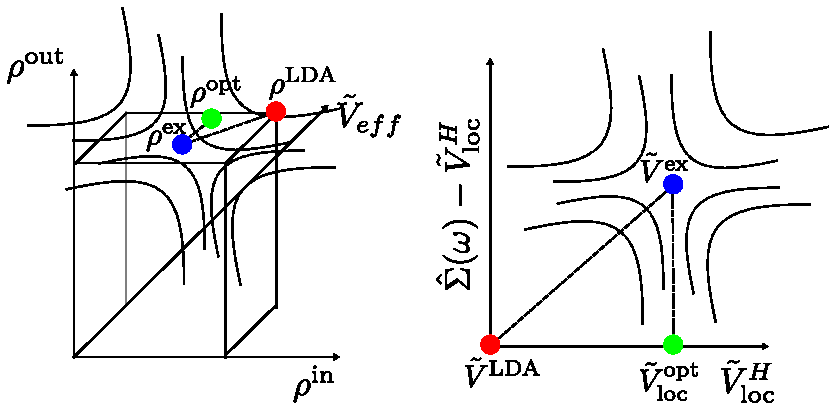
\includegraphics{./GW/HFG_space.pdf}
\caption{Schematic representation of the coordinates for the generalized
Harris-Foulkes functional. Hashed lines represent contours drawn to indicate
a saddle point. The left panel gives stationary points in the co-ordinate space
for different functionals. The blue dot indicates the stationary point for the
LDA Kohn-Sham functional with the exact density $\rho^{ex}$, 
and exact Kohn-Sham energy functional. The green dot gives a stationary point
for a hypothetical "optimal functional". The red dot is a stationary point
for the Kohn-Sham Functional using the local density approximation. 
The right panel divides the space of effective potentials into a coordinate 
composed of only local Hermitian potentials, which tend 
to be easier to work with computationally, and an orthogonal co-ordinate 
of non-Hermitian, non-local potentials, which are more problematic. 
This is in the spirit of Refs.~\cite{sohrab10, patrick12, sohrab17}. 
The figure demonstrates how one can approach an optimal
potential which minimizes the distance to the stationary point of the true interacting potential
while retaining desirable computational properties like being Hermitian and local
or allowing us to avoid multiple iterations to self-consistency.\label{hfg}}
\end{center}
\end{figure}
%
The blue dot corresponds to $\rho^{\rm ex}$, and $V^{\rm ex}_{\rm eff}$. The red dot
represents the stationary point for the HKS functional using the LDA.
Haydock \cite{haydock97} has discussed a quite general functional,
$\Phi[\{\psi_{\alpha},n(\r),V_{\rm in}(\r) \}]$. The stationary points of
this functional summarize the key features for our rigorous formulation of local methods
requires and which have been discussed up to this point.


The variation of the functional with respect to the electrons 
for the auxilliary non-interacting system is zero:
%
\begin{align}
 \frac{\delta \Phi}{\psi_{\alpha}(\r)} & = \left[-\frac{1}{2}\nabla^{2} + V_{\rm in}(\r) \right]\psi_{\alpha} -\epsilon_{\alpha}\psi_{alpha}&=& 0.
\end{align}

The variation with respect to the density leads to a connection between the effective potential
the non-interacting electronic system experiences and the exchange-correlation functional.
%
\begin{align}
 \frac{\delta \Phi}{\delta n(\r)}  & =  \frac{\delta F[n(\r)]}{\delta n(\r)} - V_{\rm in}(\r) &=& 0 \\
 \frac{\delta \Phi}{\delta V_{\rm in}(\r)} & = \sum_{\alpha}|\psi_{\alpha}|^{2} - n(\r) &=& 0
\end{align}

The stationary point of this function is minimal with respect to the basis set and
the density and maximal with respect to the effective potential $V_{\rm in}$ \cite{methfessel95}.
For an interesting demonstration of the variational properties with respect to the 
effective potential in the context of GW calculations see Ref.~\cite{sohrab10}.
%This suggests the energy functional is best used by
%first inspecting a self-consistent calculation to study what
%kind of variational degrees of freedom are needed for a
%given system. By constructing approximate functions,
%which mimic the characteristic behavior but which otherwise
%can deviate markedly, very accurate energies should
%be obtainable due to the stationary property of the functional."\cite{methfessel95}.
%It is important to stress we are also free to vary the input potential:
%\begin{equation}
%E[n_{in},V_{in}] = E_{0} + \frac{1}{2} \frac{\delta^{2}}{\delta n}\delta n_{\rm out} n_{\in} 
%\frac{1}{2}\int (V[n_{\rm in}](\r) - V_{\rm in}(\r))\delta n(\r) d\r 
%\end{equation}
%The combined functional is variational and it is {\emph minimal} with respect to the density
%and {\emph maximal} with respect to the potential. See Ismail-Beigi\cite{sohrab10} and 

Before we conclude this chapter we will introduce some diagrammatic representations introduced
by Methfessel which may help the reader picture what we have discussed\cite{methfessel95}.
We extend these diagrams so that we can show the importance of incorporating some knowledge of 
the materials dielectric properties into a calculation:
%
\[\xymatrix{
&             &                   &                 &   \cdots \ar[r]     &       n^{2}_{m+1} = n^{1}_{m+1} + \chi(V^{1}_{m+1} - V^{1}_{m}) \ar[r]  & V^{2}_{m+1} \ar[r] & \cdots \\
&             & \cdots \ar[r] & n^{1}_{m}=n^{0}_{m} + \chi(V^{0}_{m} - V^{0}_{m-1}) \ar[r] & V^{1}_{m} \ar[r] \ar[ur] & n^{1}_{m+1} \ar[u] \ar[r] & V^{1}_{m+1} \ar[ul] \ar[r] & \cdots \\
\cdots \ar[r] & n^{0}_{m-1} \ar[r] & V^{0}_{m-1} \ar[ur] \ar[r] & n^{0}_{m}\ar[u] \ar[r] & V^{0}_{m} \ar[ul] \ar[r] & \cdots &  & \\
}
\]
%
The subscript represents the iteration number and the superscript represents `the stage of mixing'. 
These sort of diagrams bare a resemblance to exact sequences \cite{whitehead50} in algebraic topology.
One does not typically have $\chi$
fully calculated and to hand so, initially, some approximation is required.
One approximation to $\chi$ could be a simple 
scalar (linear mixing) of the input and output density at a given potential. 
Another more sophisticate approach exploits Broyden's technique which allows 
us to build an estimate of $\chi$
from the observed variations in the total density and potentials.
The chain continues until it stabilizes at 
$n^{i}_{m+1}=n^{i}_{m}$ or an equivalent condition for the potential.
In practice without any mixing the bottom chain, $n^{0}_{m}$, with no density mixing, 
may never stabilize. 
Working out the optimal way of approximating and storing $\chi$ plays an important role
in enabling large scale ab initio simulations \cite{vanderbilt84, johnson88}.

The sequence of potentials and densities may also be wrapped around on itself:
%
\[\xymatrix{
	V \ar[r] & n_{\rm out}[V] \ar[r] & \hat{P}_{n_{\rm out}}[V] \ar[d] \\
	\hat{P}_{v}[V_{\rm eff}[n]] \ar[u] & V_{\rm eff}[n] \ar[l] & n\ar[l] \\
}
\]

In this sequence two projections, $\hat{P}_{n}$ and $\hat{P}_{V}$, which 
act on the density and the potential have been inserted. 
The hope is that these projection operations allow us to project the ab initio
data onto a restricted subspace which will preserve as much of the 
exactness of the original sequence as possible. 
Obtaining this local representation will be an important 
step towards forming a basis for our recursion calculations.

\section{Conclusion}
\noindent
This chapter began by introducing the Hohenberg-Kohn theorem. 
We then discussed the practical means of performing
ab initio calculations using the Kohn-Sham system and the local density
approximation. The $GW$ approximation was introduced as a way of formally
improving the density functional model according to a physically motivated
perturbation expansion.

The Harris-Foulkes discussion provides the justification for a mapping procedure
of ab initio data onto a restricted space more amenable to recursive
calculations.

Finally we discussed some interesting properties of total 
energy functionals. The hope is that the reader will see there is a wider
scope for interpreting total energy functionals than simply iterating the Kohn-Sham LDA
system to self-consistency over and over again. The input and output density, 
the effective potential, and the dielectric properties of the system are all 
related to each other.

For a given configuration of atoms it is now commonplace to send a 
DFT or $GW$ calculation off to a computing machine and within a few minutes, hours, or 
days (depending on the size of the system) come back to directories 
full of eigenvalues, charge densities, wavefunctions, forces, and total energies.
The formal transformation from these  \textit{global}, total energy methods 
based on the LDA and GW, to \textit{local representations} amenable 
to a description in terms of interatomic bonds and 
recursion type calculations has been initiated in this chapter. We
will put it into practice in the next.
